\mode*
\begin{frame}[plain,t,label=exp_capas]
  \transduration<1->{5}
  \hspace*{-0.8cm}\parbox[t]{\textwidth}{
    \only<1->{\vspace*{-0.4cm}\hspace*{-1.5cm}
      \colorbox{blueun}{
        \parbox[t][1.5cm][c]{\paperwidth}{
          \textcolor{white}{\Large\quad{DETALLE DE LOS OBJETIVOS GENERALES}}
        }
      }
    }\setbeamercovered{transparent}
    \only<1>{
      \begin{center}
        \parbox[c][2.0cm][c]{4cm}{}
      \end{center}
    }
    \only<2>{
      \begin{center}
        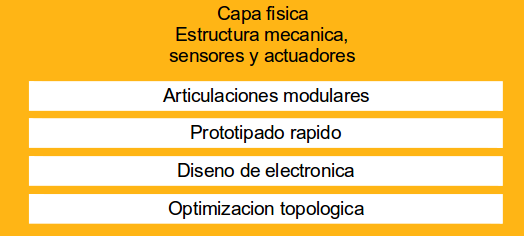
\includegraphics[height=2.0cm]{../images/objCapaFisica.png}
      \end{center}
    }
    \only<3>{
      \begin{center}
        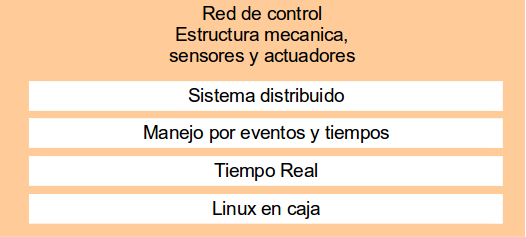
\includegraphics[height=2.0cm]{../images/objCapaRAS.png}
      \end{center}
    }
    \only<4>{
      \begin{center}
        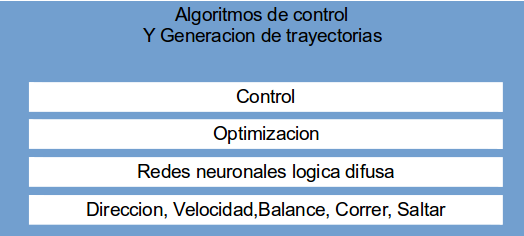
\includegraphics[height=2.0cm]{../images/objCapaControl.png}
      \end{center}
    }
    \only<5>{
      \begin{center}
        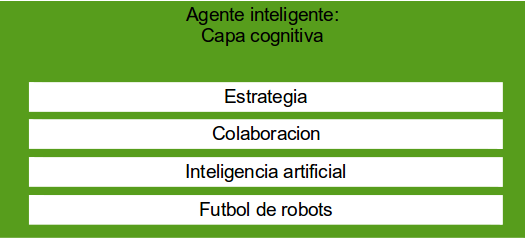
\includegraphics[height=2.0cm]{../images/objCapaCognitiva.png}
      \end{center}
    }\vspace{-0.2cm}\hspace{-1.0cm}
    \parbox[c]{12cm}{
      \begin{enumerate}[<+-|alert@+|uncover@+>][\textbf{OE:} 1.]\scriptsize
      \item Modelar, simular, analizar y sintetizar mecanismos subactuados que optimicen la energ\'ia para la locomoci\'on de caminar, saltar o correr
      \item Dise\~nar y construir una plataforma rob\'otica modular y para prototipado, capaz de configurar cadenas cinem\'aticas  controladas y/o monitoreadas bajo el sistema distribuido
      \item Implementar un sistema distribuido de sensores y actuadores que funcione en tiempo-real, bajo el principio de manejo por disparo-de-eventos y/o manejo por disparo-por-tiempos
      \item Dise\~nar, simular e implementar diferentes controles de locomoci\'on inspirados en las nuevas tendencias de investigaci\'on de caminadores sobre plataformas rob\'oticas modulares construidas
      \item Dise\~nar, simular e implementar estrategias y actividades colaborativas usando una red de caminadores
      \end{enumerate}
    }
  }
  \hyperlink{def_objesp}{\beamerreturnbutton{Volver al Objetivos Espec\'ificos}}
\end{frame}